\section{Numerical results}
\label{sec:results}

We distinguish a historical industrial experiment recorded in a research note
from a reproduced characterisation of the shell solver outputs. The former
motivates the distributional task; the latter checks the implemented data
construction before a learned model is evaluated on it.

\subsection{Injection-moulded warpage (SAOI)}
\label{sec:results:saoi}

\subsubsection{Task and evidence boundary}
The local September 2026 SAOI research note records three held-out parts, each
with 125 reference realisations and 2000 generated draws. Its quantity of
interest is final-step peak-to-valley $z$ displacement,
$\max_i u_{z,i}-\min_i u_{z,i}$. The reported Wasserstein and mean errors are
normalised by the reference quantity's standard deviation; the dispersion
ratio is $\mathrm{sd}_{\mathrm{gen}}/\mathrm{sd}_{\mathrm{ref}}$.

These numbers are reproduced from the note's tables, not recomputed from
predictions: the original SAOI HDF5 files, prediction archives and complete
historical run configurations are absent from the source tree audited for this
draft. The current \texttt{SAOI\_sweep} profiles describe replacement full
factorial experiments and must not be used as provenance for this older
fractional factorial. The historical interpretation is therefore conditional
on the note's stated data grouping and preprocessing. In particular, 125
realisations estimate a conditional law; they do not specify it exactly.

\subsubsection{Recorded comparison}
The note describes eight planned arms per model at 1000 epochs, with four
factors in a $2^{4-1}$ fractional factorial. For MGN-V these were latent
conditioning, encoder-gradient coupling, capacity and MMD weight; for
cHI-MGNflow they were batch size, flow-time sampling, capacity and learning
rate. One MGN-V arm failed during training, leaving seven recorded results.
No replicated training-seed uncertainty or convergence study accompanies the
table. Shared architectural components do not make this a controlled ablation
of stochasticity placement alone: the two objectives, capacities and tuning
factors also differ.

\begin{table}[tbp]
\centering
\caption{Historical SAOI note, mean over three parts. These are recorded
summary values, not a reproduction from raw predictions. Lower $W_1/\mathrm{sd}$
is better; dispersion ratio one matches the reference width but does not by
itself establish calibration.}
\label{tab:saoi-best}
\begin{tabular}{llccc}
\toprule
model & arm & $W_1/\mathrm{sd}$ & $|\Delta\mathrm{mean}|/\mathrm{sd}$ & dispersion ratio \\
\midrule
MeshGraphNets-V & 7 & 0.410 & 0.218 & 0.475 \\
MeshGraphNets-V & 3 & 0.434 & 0.176 & 0.526 \\
cHI-MGNflow & 1 & 0.896 & 0.724 & 0.475 \\
\bottomrule
\end{tabular}
\end{table}

The ratio of the two best recorded distances is $0.896/0.410\approx2.2$.
Across the available arms, MGN-V spans $0.410$--$0.510$ and cHI-MGNflow spans
$0.896$--$1.604$. These observed ranges do not overlap; this is not a confidence
interval or a claim about untested hyperparameters or additional geometries.

\begin{figure}[tbp]
\centering
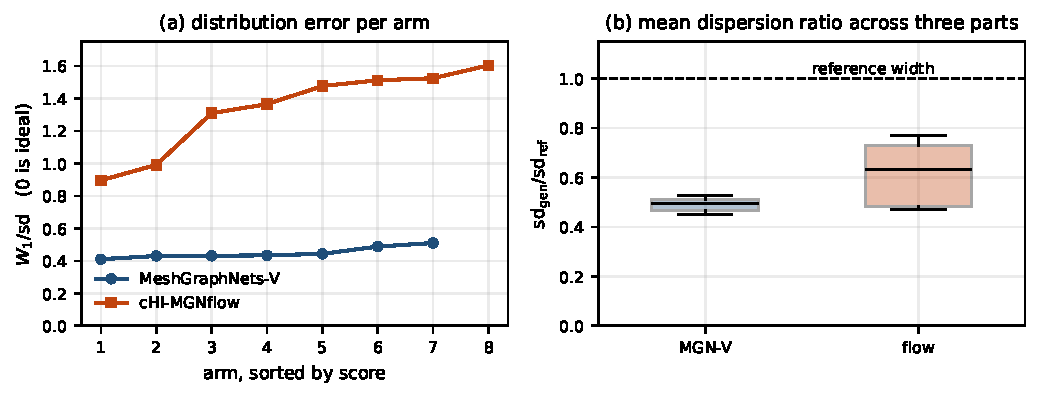
\includegraphics[width=\linewidth]{figures/saoi_ranking.pdf}
\caption{Recorded SAOI arm summaries. Each point or boxplot entry is an arm's
mean over three parts; variation across arms is not training-seed uncertainty.}
\label{fig:saoi-ranking}
\end{figure}

\subsubsection{Location and dispersion}
The note reports particularly large location errors for cHI-MGNflow on
SM-L345U-MAIN: arm 1 has normalised $W_1=1.425$ and signed mean error $1.408$;
arm 7 has $3.659$ and $3.641$. A location error is itself a distributional
calibration defect. Opposite bias signs on different parts do not rule out a
normalisation or preprocessing error; diagnosing the cause requires the
missing raw inputs, predictions and normalisers.

The largest mean dispersion ratio in the table is $0.769$ for cHI-MGNflow;
MGN-V's largest is $0.526$. The former also has per-part ratios above one on
SM-L345U-MAIN, so the average deficit must not be described as uniform across
all parts. Matching neither location nor width is a concern for tolerance
analysis, but failure probabilities depend on thresholds and tail shape and
were not measured here.

\begin{figure}[tbp]
\centering
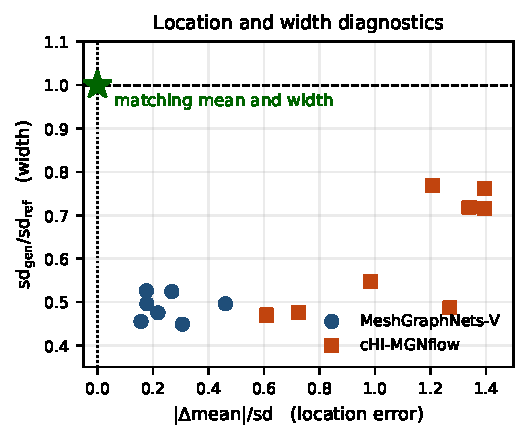
\includegraphics[width=0.60\linewidth]{figures/failure_modes.pdf}
\caption{Recorded location and width diagnostics, averaged over the three
parts for each arm. Agreement in these two moments would still leave the
distribution's shape and field dependence untested.}
\label{fig:failure-modes}
\end{figure}

\subsubsection{Factor effects and limitations}
\label{sec:results:limits}
The note's cHI-MGNflow factor contrasts are $0.333$ for flow-time sampling
(uniform lower), $0.288$ for batch size (16 lower than 32), $0.083$ for
learning rate and $0.074$ for capacity. At fixed epochs, batch size also
changes the number of optimiser updates. The largest MGN-V contrast is
$0.054$ for capacity; its encoder-gradient contrast is only $0.001$.
The missing arm breaks the balanced design, and neither sweep has replication
to distinguish these contrasts from training variability or aliased effects.
Consequently the small encoder-gradient contrast does not prove a null effect
or rule out an intervention, and the flow-time contrast does not establish a
general rule about mesh fields versus images.

The Gaussian example in Section~\ref{sec:method:shrink} distinguishes two
objectives mathematically. It does not diagnose the cause of these historical
dispersion deficits. Reproducing the SAOI evaluation requires restoring the
original data, model states, run configurations and prediction archives.

\subsection{Shell benchmark with a known withheld variable}
\label{sec:results:buckling}

\begin{figure}[tbp]
\centering
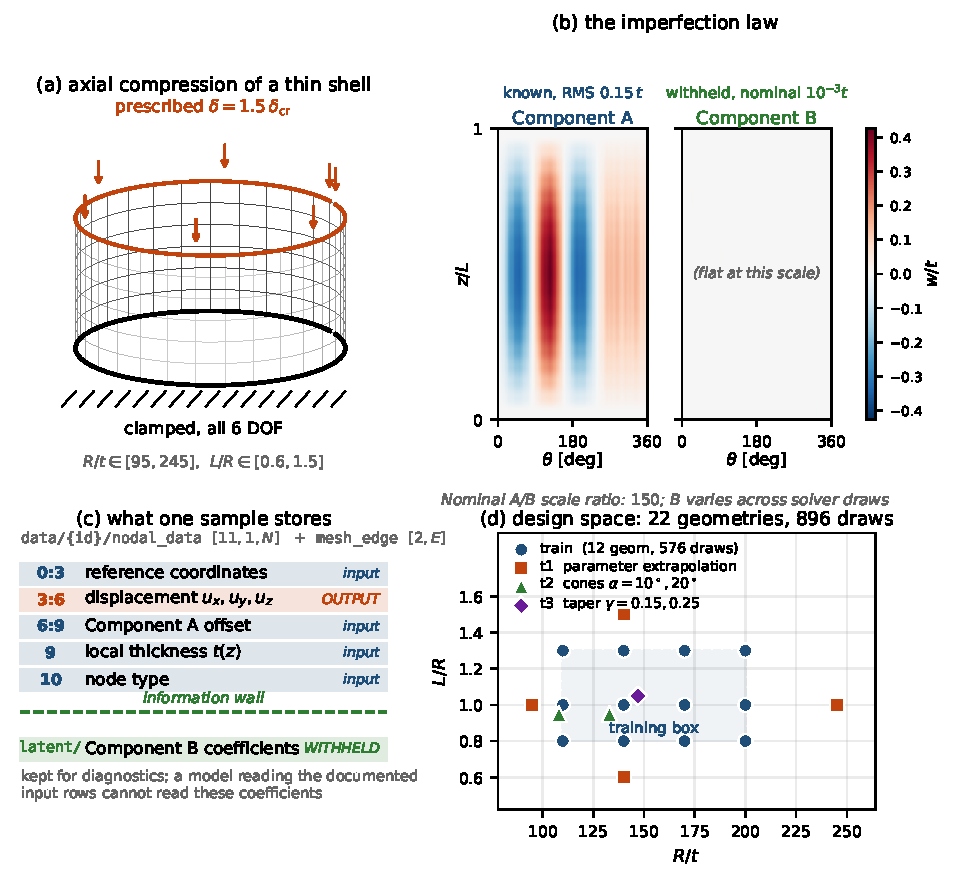
\includegraphics[width=\linewidth]{figures/dataset_overview.pdf}
\caption{Implemented construction: axial compression; deterministic and
withheld imperfection components on a common colour scale; the static HDF5
contract; and the planned geometry tiers. The setup mesh is generated at a
coarser resolution for illustration. Of eleven stored rows, eight provide
visible geometry/conditions and three hold targets that static loaders zero
in the state input. The nominal A-to-B scale ratio is 150; B's realised RMS
varies. Coincident design markers are offset for legibility.}
\label{fig:dataset}
\end{figure}

\subsubsection{Geometry, loading and imperfection law}
The implemented solver uses analytic S8R meshes, reference radius $R=1$,
elastic modulus $E=1$, Poisson ratio $0.3$ and mass density $1$ in consistent
normalised units. The base is clamped; the top is fixed transversely and in
rotation and is driven axially. The static step reaches
$0.70\,\delta_{\mathrm{cr}}$, followed by implicit dynamics over time 8 to
$1.5\,\delta_{\mathrm{cr}}$ and a hold over time 40. These are fixed solver
protocol parameters. The final displacement is a finite-time response;
equilibrium must be checked separately.

The mesh rule targets three quadratic elements per nominal half-wavelength
$1.728\sqrt{Rt}$, with integer rounding and a circumferential resonance
avoidance adjustment. This is approximately six nodal intervals per
half-wavelength, not a mesh-convergence study. The twelve training geometries
have 5311--15190 nodes. The line $0.86\sqrt{R/t}$ is the implementation's
empirical mode reference, used also to guard the signature harmonics; it is
not an independently derived classical buckling prediction.

Component A is a deterministic sum of circumferential harmonics with a
$\sin(\pi z/L)$ envelope. Harmonics within three wavenumbers of the empirical
reference are removed, and the sampled nodal RMS is normalised to $0.15t$.
It is identical across draws of a geometry. Component B uses a Mat\'ern-shaped
spectral density with nominal scale $10^{-3}t$, length parameter
$0.70\sqrt{Rt}$ and smoothness parameter $1.5$. The implementation draws
independent uniform Fourier phases with fixed spectral amplitudes and takes
the real part of the sum over a rectangular frequency truncation. It is not
an exact Gaussian Mat\'ern field or an exactly normalised RMS realisation.
The axial field is defined on a padded length $2L$ and cropped to the shell.
Archived coefficients are float32, so later evaluation avoids interpolation
but does not reproduce the original float64 field bit-for-bit.

The nominal scale ratio $0.15/10^{-3}=150$ expresses how small B is relative
to the supplied signature. Its consequences are measured on the solver
outputs, rather than asserting that B is the only possible numerical source
of branch selection. The non-axisymmetric A and the discrete mesh also
preclude an assertion of exact rotational symmetry of the conditional law.

\subsubsection{Plan and model-visible contract}
\begin{table}[tbp]
\centering
\caption{Planned dataset. Counts precede quality filtering. Tiers t1--t3 are
held out from model fitting. Remaining inside the training interval of local
$R/t$ reduces one extrapolation confound; it does not isolate every geometric
or discretisation effect.}
\label{tab:buckling-tiers}
\begin{tabular}{llrrl}
\toprule
tier & family & geometries & draws & local $R/t$ \\
\midrule
train & cylinders & 12 & 576 & 110--200 \\
t1 & cylinders & 4 & 128 & 95, 140, 245 \\
t2 & cones, $10^\circ$/$20^\circ$ & 4 & 128 & approximately 115--191 \\
t3 & sinusoidal thickness variation & 2 & 64 & approximately 112--140 \\
\bottomrule
\end{tabular}
\end{table}

The shared HDF5 layout is $[11,1,N]$ nodal data plus directed mesh edges.
Rows 0--2 are perfect-shell coordinates; rows 3--5 are displacements measured
from the imperfect starting surface; rows 6--8 are the known A offset;
row 9 explicitly supplies local thickness $t(z)$ in the reference length
units; row 10 is the boundary node type. Thus \texttt{input\_var=3},
\texttt{output\_var=3}, and \texttt{cond\_var=5}. This is a static
condition-to-terminal-field task with one stored frame. The state input is
zeroed by the static loader; copying its stored target rows into the input
would invalidate the withholding construction. The B coefficients and
outcome diagnostics are stored separately under \texttt{latent/} and in
metadata, and must not become model features.

An audit corrected the taper deck: the original writer supplied uniform
thickness even when the plan specified $t(z)$. The corrected writer supplies
nodal thickness, and the generator and exporter reject legacy taper archives
without matching versioned solve settings. The export also requires an
explicit plan and tier selection, since the training loaders do not enforce
tier metadata. A random within-file split is not a geometry-holdout test.

\subsubsection{Reproduced characterisation}
The immutable source snapshot captured on 13 September 2026 at 07:32 KST
contains $\SnapshotDraws$ returned solver-success records and
$\SnapshotFailures$ returned failure records. It includes the complete
training tier, $\TrainDraws$ draws over twelve geometries, and 254
non-training draws. It is an explicitly dated snapshot, not the current
generator progress. Input hashes and per-geometry measurements accompany
this draft; all displacement, radial-field and stored-spectrum relationships
were recomputed from the archives.

\begin{figure}[tbp]
\centering
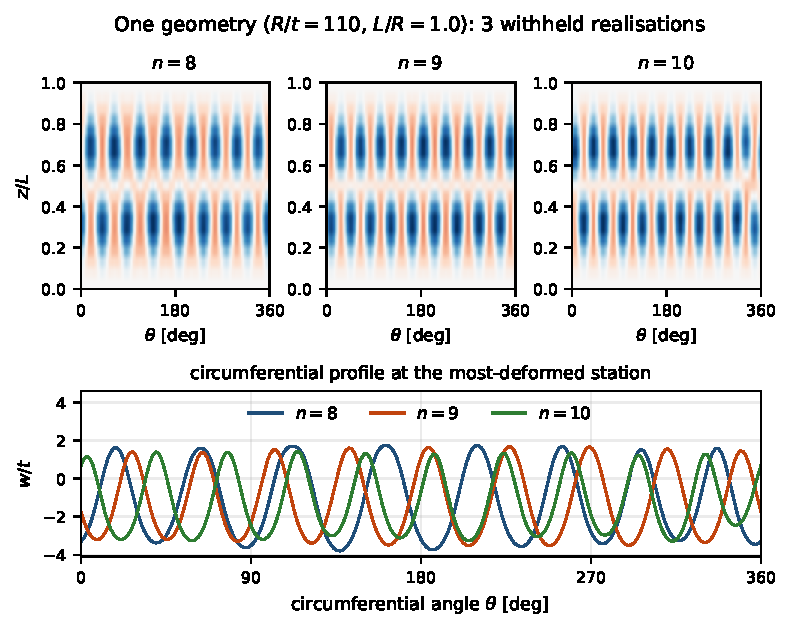
\includegraphics[width=0.82\linewidth]{figures/buckling_fields.pdf}
\caption{Three selected draws at $R/t=110$, $L/R=1.0$, one per observed
dominant mode. Top: radial displacement divided by nominal thickness, with
an individual colour range per panel. Bottom: circumferential profiles at
the respective maximum-response axial stations. Selection illustrates modes,
not their probabilities; the frequency distributions are shown separately.}
\label{fig:buckling-fields}
\end{figure}

\begin{figure}[tbp]
\centering
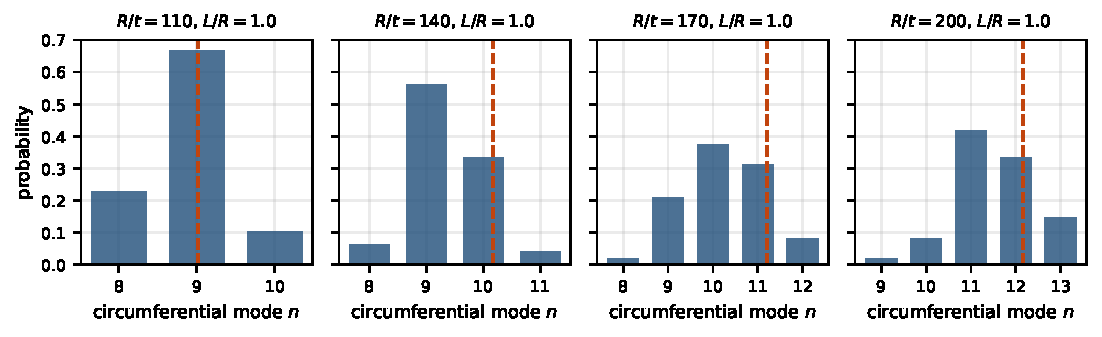
\includegraphics[width=\linewidth]{figures/buckling_modes.pdf}
\caption{Unfiltered finite-time outcomes at fixed $L/R=1.0$, 48 draws per
geometry. Dashed lines show the empirical reference $0.86\sqrt{R/t}$.
All panels use the frozen training-tier records.}
\label{fig:buckling-modes}
\end{figure}

Across the twelve training geometries, the dominant-mode label takes
$\TrainModesMin$--$\TrainModesMax$ distinct values and the largest mode share
is $\TrainTopMin$--$\TrainTopMax\%$. The mean observed mode lies below the
empirical reference by 1.6--13.1\%. These are measured finite-time label
frequencies; no eigenvalue-spectrum or equilibrium study here establishes
the mechanism behind their changes.

The recorded drift is the range of radial RMS divided by its mean over the
last third of saved displacement blocks. Of the training draws,
$\TrainDriftFailures/\TrainDraws$ ($\TrainDriftPercent\%$) exceed 0.15.
For $L/R=0.8$, 1.0 and 1.3, the exceedance counts are respectively 0, 22 and
94 out of 192. Constant RMS can coexist with a changing field shape, so even
a low value is not a force-residual or equilibrium certificate. The raw
characterisation retains these draws and reports their drift; the default
quality-filtered HDF5 export excludes them and therefore represents a
selected subset of the original imperfection law. Both counts and rejection
reasons must accompany an export to avoid hiding this selection effect.

For a dimensionally consistent cross-geometry diagnostic, we also compare
the first 40 nonzero modes of each axially averaged magnitude spectrum after
unit-$L^2$ normalisation. The unbiased sample energy distances over the 66
unordered training-geometry pairs range from 0.030 to 1.050. This descriptor
discards amplitude, phase and axial arrangement and is distinct from the
per-station descriptor in Section~\ref{sec:protocol}. Positive empirical
distances without a sampling-uncertainty analysis do not prove statistical
separation of every pair. The full stored field contains information omitted
by either this spectrum or its argmax label; their relative usefulness for a
learned model remains to be tested.

\subsubsection{Status and remaining validation}
The contribution demonstrated here is an implemented data construction and
an audit of its outputs. No trained-model comparison, calibrated shell
surrogate, autoregressive shell rollout or persistent-latent benefit is
reported. Corrected taper runs are tracked separately from the invalid
uniform-thickness results. Stronger equilibrium claims require displacement,
force and energy convergence checks and sensitivity to the loading/settling
protocol and mesh; larger, quality-filtered samples alone cannot supply that
evidence.
